\documentclass[12pt]{article}

%-------------PACKAGES------------- 
\usepackage[margin=1in]{geometry} 
\usepackage{amsmath,amsthm,amssymb}
\usepackage{pgfplots}
\usepackage{float}
\usepackage{braket}
\usepackage{titling}
\usepackage{tikz}
\usepackage{mathtools}
\usepackage{listings}
\usepackage{color}
\usepackage{caption}
\usepackage{subcaption}
\usepackage{algorithm,algpseudocode}

%-------------FORMATTING-------------
\setlength{\droptitle}{-6em} 
\setlength{\parindent}{0pt}
 
%--------------COMMANDS--------------
\newcommand{\N}{\mathbb{N}}
\newcommand{\Z}{\mathbb{Z}}
\newcommand{\R}{\mathbb{R}}
\newcommand{\C}{\mathbb{C}}
%\renewcommand{\qedsymbol}{\filledbox}

\DeclarePairedDelimiter \abs{\lvert}{\rvert}%
\DeclarePairedDelimiter \norm{\lVert}{\rVert}%

%------------ENVIRONMENTS------------- 
\newenvironment{theorem}[2][]{\begin{trivlist}
\item[{\bfseries #1}\hskip \labelsep {\bfseries #2.}]}{\end{trivlist}}
\newenvironment{lemma}[2][Lemma]{\begin{trivlist}
\item[\hskip \labelsep {\bfseries #1}\hskip \labelsep {\bfseries #2.}]}{\end{trivlist}}
\newenvironment{exercise}[2][Exercise]{\begin{trivlist}
\item[\hskip \labelsep {\bfseries #1}\hskip \labelsep {\bfseries #2.}]}{\end{trivlist}}
\newenvironment{reflection}[2][Reflection]{\begin{trivlist}
\item[\hskip \labelsep {\bfseries #1}\hskip \labelsep {\bfseries #2.}]}{\end{trivlist}}
\newenvironment{proposition}[2][Proposition]{\begin{trivlist}
\item[\hskip \labelsep {\bfseries #1}\hskip \labelsep {\bfseries #2.}]}{\end{trivlist}}
\newenvironment{corollary}[2][Corollary]{\begin{trivlist}
\item[\hskip \labelsep {\bfseries #1}\hskip \labelsep {\bfseries #2.}]}{\end{trivlist}}
\theoremstyle{remark}
\newtheorem*{remark}{Remark}

%-------------CODE-STYLE------------
\definecolor{dkgreen}{rgb}{0,0.6,0}
\definecolor{gray}{rgb}{0.5,0.5,0.5}
\definecolor{mauve}{rgb}{0.58,0,0.82}
\lstset{frame=tb,
	language=C++,
	aboveskip=3mm,
	belowskip=3mm,
	showstringspaces=false,
	columns=flexible,
	basicstyle={\small\ttfamily},
	numbers=none,
	numberstyle=\tiny\color{gray},
	keywordstyle=\color{blue},
	commentstyle=\color{dkgreen},
	stringstyle=\color{mauve},
	breaklines=true,
	breakatwhitespace=true,
	tabsize=3
}

\lstset{
	morekeywords={end}
}

%------------------------------------ 
%---------START-OF-DOCUMENT----------
%------------------------------------

\begin{document}
 
\title{Homework 6}
\author{David Miller \\ 
MAP5345: Partial Differential Equations I} 
 
\maketitle

\section*{Problem 1}

\textit{Classify each PDE as linear or nonlinear and homogeneous or nonhomogeneous. If the PDE is linear, rewrite it in canonical form $\mathcal{L}[u] = g(x)$, where $\mathcal{L}$ is a linear operator and $g(x)$ is the inhomogeneous term (which depends only on the independent variable $x$).} \\ \\
\textit{a) $u_t = yu_{xx} + t^2sin(xy)u_yy$} \\ 

Linear: $\mathcal{L} = (\partial_t - y\partial_{xx} - yt^2sin(xy)\partial_y), \quad g(x) = 0$ \\
Homogeneous: $u \equiv 0 \Rightarrow u_t - yu_{xx} -yt^2sin(xy)u_y = 0$ \\

\textit{b) $v_t + 2v_xv_{xxx} = kv_{xx}$} \\

Linear: $\mathcal{L} = (\partial_t + 2\partial_x\partial_{xxx} - k\partial_{xx}), \quad g(x) = 0$ \\
Homogeneous: $ \equiv 0 \Rightarrow v_t - 2v_xv_{xxx} - kv_{xx} = 0$ \\

\textit{c) $h_{xx} + 2h_{yy} + 3x^2e^{-y} = 0$}\\ 

Linear: $\mathcal{L} = (\partial_{xx} + \partial_{yy}), \quad g(x) = -3x^2e^{-y}$ \\
Nonhomogenous: $h \equiv 0 \Rightarrow h_{xx} + 2h_{yy} + 3x^2e^{-y} = 3x^2e^{-y}$ \\

\textit{d) $u_t + cos(u_x) = 0$} \\ 

Nonlinear \\
Nonhomogeneous: $u \equiv 0 \Rightarrow u_t + cos(u_x) = 1$

\pagebreak

\section*{Problem 2}

\textit{Consider a PDE for $u(x,t)$. Can you come up with an inhomogeneous PDE that seems to be homogeneous according to the undergraduate definition? This seems to contradict the canonical form of linear PDEs from class, but why is there actually no contradiction?} \\

A simple inhomogeneous PDE that satisfies the undergraduate definition of homogeneous is 
$$ u_{tt} + u_{xx} - cosh(u) = 0. $$

The trivial solution $u \equiv 0$ does not solve the PDE so it is not homogeneous. This seems to contradict the canonical form of PDEs but it does not. This is because it is not linear. In fact the undergraduate way to determine if a PDE is homogeneous always works for linear PDEs because the trivial solution is always a solution to linear PDEs and therefore this does not contradict the canonical form. However the undergraduate method could be wrong when the PDE is not linear, but in this case there is no canonical form so there is no contradiction.

\pagebreak

\section*{Problem 3}

\textit{Consider the PDE for $\eta(x,t)$}
\begin{align}
	\eta_t + \eta\eta_x = 0
\end{align}
\textit{Since the PDE is nonlinear, it should not be possible to combine solutions in general. Suppose that $u(x,t)$ and $v(x,t)$ are solutions to the above PDE.} \\ \\
\textit{a) Try to prove that $w(x,t) = au(x,t) + bv(x,t)$ is also a solution (for $a,b \in \mathbb{R}$), and explain where the proof fails.} \\

Assuming $w$ is a solution to (1) then we get
\begin{align*}
	w_t + ww_x & = (au_t + bv_t) + (au + bv)(au_x + bv_x) \\
	& = au_t + bv_t + a^2uu_x + b^2vv_x + abuv_x + abvu_x
\end{align*}

It is evident that the above is not equal to $(u_t + v_t) + (uu_x + vv_x)$. One might try to mess around with $a$ and $b$ to create a solution but they are arbitrary constants so trying to do so will violate the concept of an arbitrary linear solution. \\

\textit{b) Now, suppose that there is at least one non-trivial solution $u(x,t)$ to the PDE. What is the simplest counterexample that you can construct to prove that the PDE above is not linear.} \\ 

Let $u = x - 1$ and $v = 1-t$. Clearly they individually solve the PDE but $w = au + bv = ax - bt$ does not. We can quickly show this by
\begin{align*}
	w_t + ww_x = -b + a^2x - abt 
\end{align*}
Again we see that this is clearly not zero unless we mess with $a$ and $b$ which contradicts the definition of arbitrary linear solution. 

\pagebreak

\section*{Problem 4}

\textit{Consider an operator $\mathcal{L}$ that acts on a function $u(x,t)$ via}
\begin{align}
	\mathcal{L}[u] = xt^2u_t + e^{-x}u_{xx}
\end{align}
\textit{According to the class, this is a linear operator and thus it should be true that $\mathcal{L}[au+bv] = a\mathcal{L}[u] + b\mathcal{L}[v]$ for all functions $u$ and $v$ and real numbers $a$ and $b$. Verify this equality directly.} \\ 

Directly evaluating we get
\begin{align*}
	{L}[au+bv] & = xt^2\partial_t(au + bv) + e^-x\partial_{xx}(au + bv) \\
	& = xt^2(au_t + bv_t) + e^{-x}(au_{xx} + bv_{xx}) \\
	& = a(xt^2u_t + e^{-x}u_{xx}) + b(xt^2v_t + e^{-x}v_{xx}) \\
	& = a\mathcal{L}[u] + b\mathcal{L}[v]
\end{align*}
which shows that (2) is a linear operator.

\pagebreak

\section*{Problem 5}

\textit{Consider a long, narrow gas chamber of length $L$. We aim to determine the concentration of oxygen $u(x,t)$ inside the chamber, as governed by the diffusion equation. The left side of the chamber is in contact with a source of pure oxygen, so that $u(0,t) = 1$ at all times. The right side is in contact with the atmosphere, so $u(L,t) = 0.21$ at all times (atmospheric level of oxygen). Initially, the concentration of oxygen in the chamber is equal to the atmospheric value $u(x,0) = 0.21$. Solve for $u(x,t)$ and graph the solution with Julia.} \\ 

Since we do not have homogeneous Dirichlet boundary conditions we can not apply separation of variables to find our solution. Instead we will assume that we have the following solution form
$$ u(x,t) = u^H(x,t) + u^P(x,t) $$
where $u^(x,t)$ is the homogeneous solution and $u^P(x,t)$ is the particular solution. We can do this because the diffusion equation is linear and we assume $u^H$ and $u^P$ solve the PDE. We already know from our homeworks that the general solution for homogeneous Dirichlet conditions is 
$$ u^H(x,t) = \sum\limits_{n=1}^\infty A_ne^{-\lambda kt}sin(\frac{n\pi x}{L}) $$
for some constant $A$. Now we need to find $u^P$ that solves the PDE and satisfies the boundary conditions since $u^H(0,t) = u^H(L,t) = 0$. The simplest particular solution is 
$$ u^P(x,t) = u(0,t) - \frac{.21 - 1}{L}x = 1 - \frac{.79}{L}x $$
which can be checked easily to solve the PDE. Putting all this together we get that
\begin{align}
	u(x,t) = 1 - \frac{.79}{L}x + \sum\limits_{n=1}^\infty A_ne^{-\lambda kt}sin(\frac{n\pi x}{L})
\end{align}
where $\lim\limits_{t \rightarrow \infty} \rightarrow u^P(x,t)$ as desired. Relabeling $sin(\frac{n\pi x}{L})$ as $X_n$ and applying initial condition we get
\begin{align*}
u_0 = 1 - \frac{.79}{L}x = \sum\limits_{n=1}^\infty A_nX_n	
\end{align*} 
which we can use to solve for $A_n$. What we do is move $u^P(x,t)$ to the LHS and take the inner product of both sides with respect to eigenfunction $X_m$. 
\begin{align*}
	\braket{u_0 - u^P, X_m} = \sum\limits_{n=1}^\infty \braket{A_nX_n, X_m} = \sum\limits_{n=1}^\infty A_n\braket{X_n, X_m}
\end{align*}
From previous homeworks we already know that $\braket{X_n, X_n} = \frac{L}{2}$ if $m = n$ and 0 otherwise. Multiplying by $\frac{2}{L}$ on both sides allows us to solve for $A_n$
\begin{align*}
	A_n & = \frac{\braket{u_0 - u^P, X_n}}{\braket{X_n, X_n}} \\
	& = \frac{2}{L}\int\limits_0^L (u_0 - u^P)X_n \, dx \\
	& = \frac{2}{L}\int\limits_0^L (0.21 - 1 + \frac{.79}{L}x)sin(\frac{n\pi x}{L}) \, dx \\
	& = -\frac{2}{L}\int\limits_0^L .79sin(\frac{n\pi x}{L}) \, dx + \frac{2}{L}\int\limits_0^L \frac{.79x}{L}xsin(\frac{n\pi x}{L}) \, dx \\
	& = \frac{1.58}{n\pi}cos(\frac{n\pi x}{L})\bigg\vert_0^L + \frac{1.58}{L^2}\bigg(-\frac{xL}{n\pi}cos(\frac{n\pi x}{L})\bigg\vert_0^L + \frac{L}{n\pi}\int\limits_0^L cos(\frac{n\pi x}{L}) \, dx\bigg) \\
	& = -\frac{1.58}{n\pi}
\end{align*}
Putting all this together we get the solution to our PDE
\begin{align*}
	\fbox{$u(x,t) = 1 - \frac{.79}{L}x + \sum\limits_{n=1}^\infty A_ne^{-\lambda kt}sin(\frac{n\pi x}{L}), \quad A_n = -\frac{1.58}{n\pi}$}
\end{align*}

The graphs below have $k = 0.5$ and $L = 5$. However we are on a computer so we can not plot the exact solution, but instead we are plotting
$$ \tilde{u}(x,t) = 1 - \frac{.79}{L}x + \sum\limits_{n=1}^\N A_ne^{-\lambda kt}sin(\frac{n\pi x}{L}), \quad A_n = -\frac{1.58}{n\pi} $$

for some truncation value $N$. We can clearly see from the graphs $\lim\limits_{N\rightarrow\infty} \tilde{u}(x,t) \rightarrow u(x,t)$, which is what e expect. We also see that our system is tending towards the equilibrium concentration $u^P(x,t)$.

\pagebreak
\begin{figure}[H]
	\centering
	\begin{subfigure}{.5\textwidth}
		\centering
		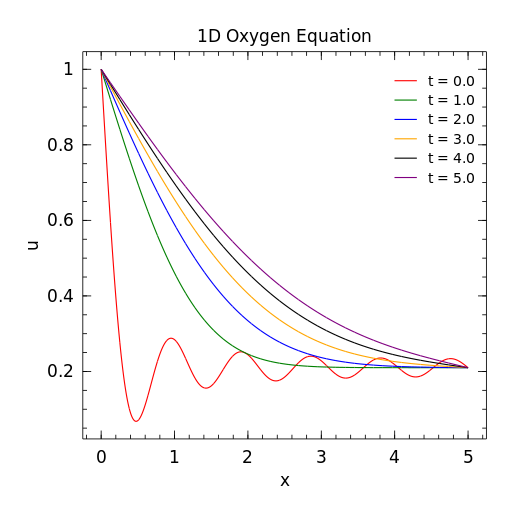
\includegraphics[width=1\linewidth]{Q5_10.png}
		\caption*{Truncation of $u(x,t)$ at $N = 10$.}
		\label{fig:sub1}
	\end{subfigure}%
	\begin{subfigure}{.5\textwidth}
		\centering
		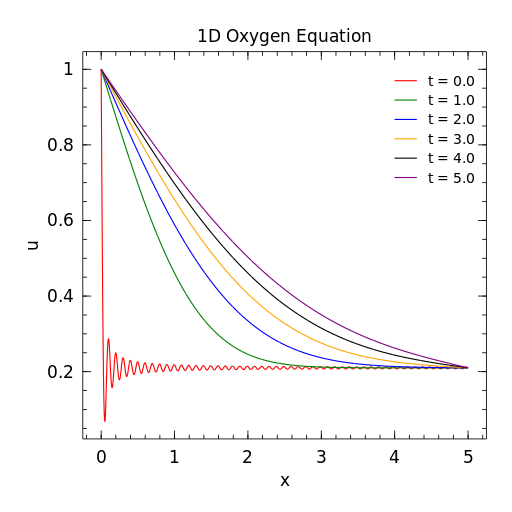
\includegraphics[width=1\linewidth]{Q5_100.png}
		\caption*{Truncation of $u(x,t)$ at $N = 100$.}
		\label{fig:sub2}
	\end{subfigure}
	\label{fig:test}
\end{figure}

\begin{figure}[H]
	\centering
	\begin{subfigure}{.5\textwidth}
		\centering
		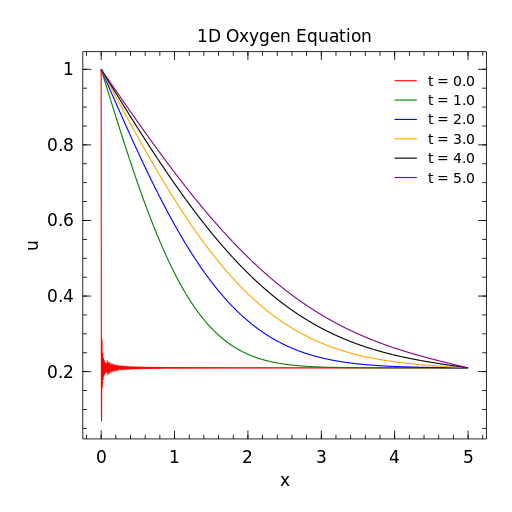
\includegraphics[width=1\linewidth]{Q5_1000.png}
		\caption*{Truncation of $u(x,t)$ at $N = 1000$.}
		\label{fig:sub1}
	\end{subfigure}%
	\begin{subfigure}{.5\textwidth}
		\centering
		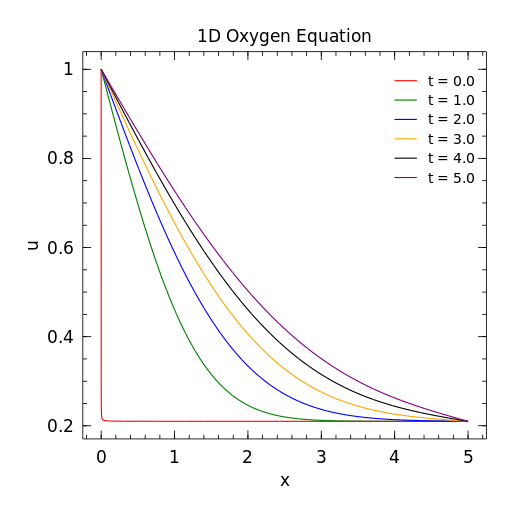
\includegraphics[width=1\linewidth]{Q5_10000.png}
		\caption*{Truncation of $u(x,t)$ at $N = 10000$.}
		\label{fig:sub2}
	\end{subfigure}
	\caption{Plots of our PDE for different truncation values, $k = 0.5$, and $L = 5$.}
	\label{fig:test}
\end{figure}

\pagebreak

\section*{Problem 6}

\textit{Consider the 1D heat equation for the temperature $u(x,t)$ in a narrow rod of length $L$. You are heating the left end $(x = 0)$ with a constant heat flux. The right ond $(x = L)$ is perfectly insulated. Solve for the temperature $u(x,t)$ by putting together all of the tricks. Graph the solution with Julia. Interpret what is happening physically. Is there a steady state?} \\

\text{NOTE: Colton and I worked on 6 together so there might be some overlap in our work. } \\

From the problem we have that
$$ u_x(0,t) = u_L, \quad u_x(L,t) = 0, \quad u(x,0) = u_0(x) $$
where $u_L$ is some constant value. Now we assume that $u(x,t)$ is some linear combination of solutions, that is
\begin{align*}
	& u(x,t) = f(x,t) + g(x,t) \\
	& g_x(0,t) = u_L, \, g_x(L,t) = 0
\end{align*} 
The simplest choice for $g_x(x,t)$ is $g_x(x,t) = -\frac{u_L}{L}x + u_L$ and therefore $g(x,t) = -\frac{u_L}{2L}x^2 + u_Lx$, where we omit the integrating constant since it still solves our conditions but we don't have to figure out another constant. Now we have
\begin{align*}
	f(x,0) = u_0(x) - g(x,0) = u_0 + \frac{u_L}{2L}x^2 - u_Lx,
\end{align*}
 and we also know that $f_x = 0$ on the boundaries since we have let $g(x,t)$ take care of the boundary conditions. Plugging all this back into the PDE we get
\begin{align*}
	& f_t(x,t) + g_t(x,t) = k(f_{xx}(x,t) + g_{xx}(x,t)) \Rightarrow f_t(x,t) = kf_{xx}(x,t) - k\frac{u_L}{L}
\end{align*}
since $g_t(x,t) = 0$ due to having no dependence on $t$. We still have an annoying $-k\frac{u_L}{L}$, so what we can do is alter $g(x,t)$ by adding an extra factor
$$ g(x,t) = -\frac{u_L}{2L}x^2 + u_Lx -k\frac{u_L}{L}t $$
where we can easily verify that this still solves the PDE and takes care of the nonhomogeneous conditions while killing off the annoying term. Then we finally arrive at a PDE we can solve
\begin{align*}
	& f_t(x,t)  = kf_{xx}(x,t) \\
	& f_x(0,t) = f_x(L,t) = 0 \\
	& f(x,0) = u_0(x) + \frac{u_L}{2L}x^2 - u_Lx
\end{align*}
{
This is a PDE we have solved in class and in homework, so the solution is 
\begin{align*}
	f(x,t) = \sum\limits_{n=0}^\infty A_n e^{ktn^2\pi^2/L^2}cos(\frac{n\pi x}{L})
\end{align*}
where we just need to solve for $A_n$. To do this we set $t = 0$ and take the inner product of both sides with $X_m - cos(\frac{m\pi x}{L})$. Doing this we get
\begin{align*}
	A_n & = \frac{\braket{f_0, X_m}}{\braket{X_n, X_m}} \\
	& = \frac{2}{L}\int\limits_0^L (u_0(x) + \frac{u_L}{2L}x^2 - u_Lx)cos(\frac{m\pi x}{L}) \, dx \hspace{5cm} {n = m \neq 0} \\
	& = -\frac{2}{n\pi}\int\limits_0^L (u^\prime_0(x) + \frac{u_L}{L}x - u_L)sin(\frac{m\pi x}{L}) \, dx \\
	& = -\frac{2L}{n^2\pi^2}\bigg((u^\prime_0(x) + \frac{u_L}{L}x - u_L)cos(\frac{m\pi x}{L})\bigg)\bigg\vert_0^L + \frac{2L}{n^2\pi^2}\int\limits_0^L (u^{\prime\prime}_0(x) + \frac{u_L}{L})cos(\frac{m\pi x}{L}) \,dx \\
	& = \frac{2}{L}\braket{u^{\prime\prime}_0(x),X_m}
\end{align*}
Using the inner product of $X_m$ with itself we can then determine the coefficient $A_0$ and have a solution
\begin{align*}
	A_n  = \frac{2L}{n^2\pi^2}\braket{u^{\prime\prime}_0(x),X_m}, \quad A_0 = \frac{\braket{f_0, 1}}{L} 
\end{align*}
Plugging everything back in we finally get a solution to our original PDE
\begin{align*}
	u(x,t) = -\frac{u_L}{2L}x^2 + u_Lx - & k\frac{u_L}{L}t + A_0 + \sum\limits_{n=1}^\infty A_ne^{-ktn^2\pi^2/L^2}cos(\frac{n\pi x}{L}), \\
	 A_0 = \frac{\braket{f_0,1}}{L}, & \quad	A_n  = \frac{2L}{n^2\pi^2}\braket{u^{\prime\prime}_0(x),X_m}
\end{align*}
All that is left now is to pick a constant for $u_L$ and an appropriate $u_0(x)$ so that we can graph the solution. 
\end{document}
